% 02_background.tex  – concise (≤ 3 pp.), details in Appendix A
% ------------------------------------------------------------------
\section{Theoretical Background \& Related Work}
\label{sec:background}

\paragraph{Notation.} We denote \(T_p\) and \(T_f\) as the numbers of observed and predicted timesteps, respectively. Following UniTraj conventions~\cite{unitrajFeng2024}, agent trajectories are represented as \(\boldsymbol{X}_d \in \mathbb{R}^{N_{\max} \times T_p \times F_{ap}}\) and map polylines as \(\boldsymbol{X}_s \in \mathbb{R}^{K_{\max} \times L \times F_{map}}\), where \(N_{\max}\) is the maximum number of agents, \(K_{\max}\) is the maximum number of map polylines, \(L\) is the points per polyline, and \(F_{ap}, F_{map}\) are the respective feature dimensions. Ground truth trajectories for the center agent are denoted \(\boldsymbol{y}_c \in \mathbb{R}^{T_f \times 4}\). For rasterized approaches, BEV representations use \(H \times W\) spatial resolution with \(F_d, F_s\) channel dimensions for dynamic and static inputs, respectively. Transformer models employ \(M\) output modes, \(K\) sampling points per deformable attention query, and \(N\) attention heads. Feature pyramid networks utilize \(L\) levels indexed by \(\ell \in \{0,\dots,L-1\}\), with feature maps \(C_\ell \times H_\ell \times W_\ell\) at each level. A comprehensive symbol table is provided in Appendix~\ref{app:notation}.

%--------------------------------------------------------------------

\subsection{Scene Representation Paradigms}
\label{ssec:scene_repr}

\begin{figure}[H]
\centering
\begin{subfigure}[t]{0.35\textwidth}
    \centering
    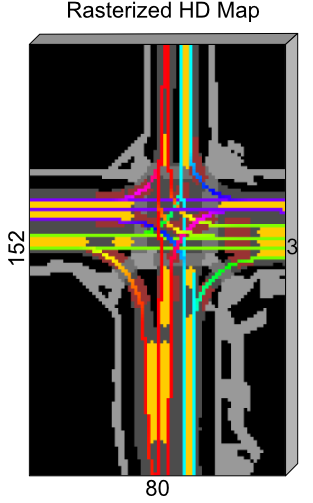
\includegraphics[width=\textwidth]{figures/caspnet-bev-repr.png}
    \caption{Rasterized BEV encoding}
    \label{fig:rasterized}
\end{subfigure}
\hfill
\begin{subfigure}[t]{0.37\textwidth}
    \centering
    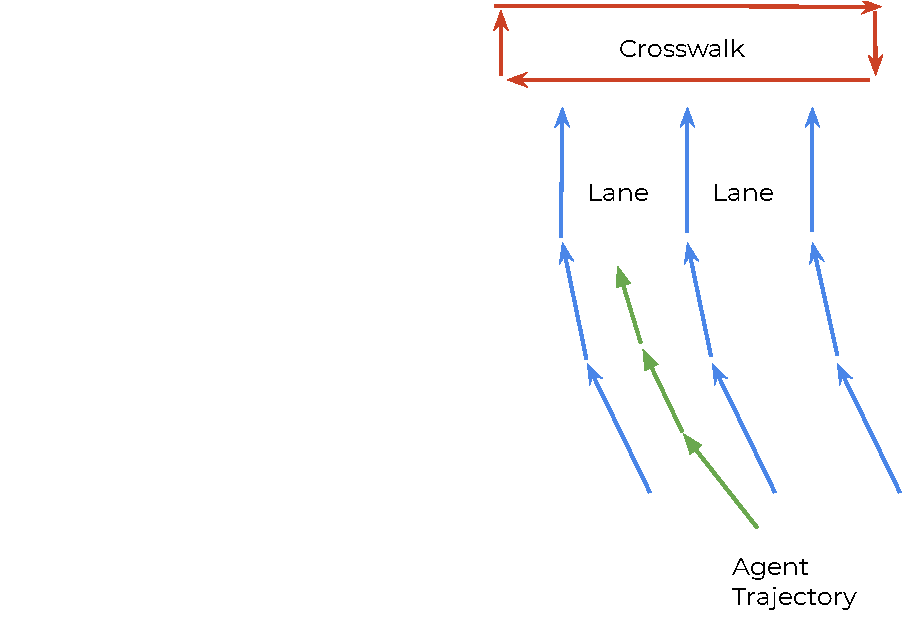
\includegraphics[width=\textwidth]{figures/vectornet-2020-vector-repr.pdf}
    \caption{Vectorized polyline preservation}
    \label{fig:vectorized}
\end{subfigure}
\caption{Scene representation paradigms in trajectory prediction: (a) rasterized approaches stack agent trajectories and HD maps into BEV images~\cite{caspnetSchäfer2022}, (b) vectorized methods preserve geometric polylines~\cite{gao2020vectornet}.}
\label{fig:scene_representations}
\end{figure}

\textbf{Raster grids.} Early systems stack past agent masks and HD-map layers into BEV images, exploiting convolutional backbones to capture local correlations while keeping runtime independent of the number of agents~\cite{cui2019multimodal,chai2019multipath}.

\textbf{Vector tokens.} Later work encodes agents and lanes as vectorized geometric primitive such as polylines, enabling graph ( LaneGCN~\cite{liang2020learning}, VectorNet~\cite{gao2020vectornet}) or transformer based (QCNet~\cite{qcnetZhou2023}, QCNeXt~\cite{qcnextZhou2023}, LMFormer~\cite{lmformerYadav2025}) approaches with higher geometric fidelity but runtime that grows with scene complexity.\\
While only \emph{agent-centric} coordinate systems allow for tractable application of rasterized scene representations, vectorized can employ a novel paradigm to represent all coordinates in a given scene. This so-called \emph{query-centric} approach will be discussed in greater detail in~\autoref{sec:qc_paradigm}.

% CASPNet embodies the \emph{raster} philosophy; CASPFormer adopts a hybrid strategy—retaining a CNN backbone for perception compatibility, but switching to a vectorized transformer decoder for output precision.

%--------------------------------------------------------------------
\subsection{Context-Aware Scene Prediction}
\label{ssec:caspnet}

This section distills the key ideas behind \emph{Context-Aware Scene Prediction Network} (CASPNet)~\cite{caspnetSchäfer2022} and its transformer successor \emph{CASPFormer}~\cite{caspformerYadav2024}. Both architectures perform \emph{joint multi-agent} trajectory forecasting from rasterized bird's-eye-view (BEV) inputs, yet they differ strongly in how they fuse context and decode trajectories. We summarize their core components, strengths, and limitations.

\subsubsection*{CASPNet: Rasterized BEV Encoding with Dual FPN}

\textbf{CASPNet}~\cite{caspnetSchäfer2022} processes rasterized BEV inputs through a dual-encoder architecture that separately handles dynamic agent trajectories and static HD map information. Overall, it strongly resembles a \emph{fully convolutional network} as it employs no fully connected layers, meaning that the spatial representation of the scene is preserved throughout the network. Furthermore, it can be classified as a \emph{feature pyramid network} (FPN)~\cite{FPNLin2017} as it provides the decoder with latent representations at multiple spatial resolutions. Together, these architectural qualities starkly resemble the famous \emph{U-Net} architecture with \emph{lateral skip connections}~\cite{UNetLSRonneberger2015}. Considering CASPNet's usage of \emph{attention} mechanisms within the skip connections its closest relative in the field of image segmentation is the \emph{Attention U-Net}~\cite{AttentionUNetOktay2018}.

\begin{figure}[ht]
  \centering
  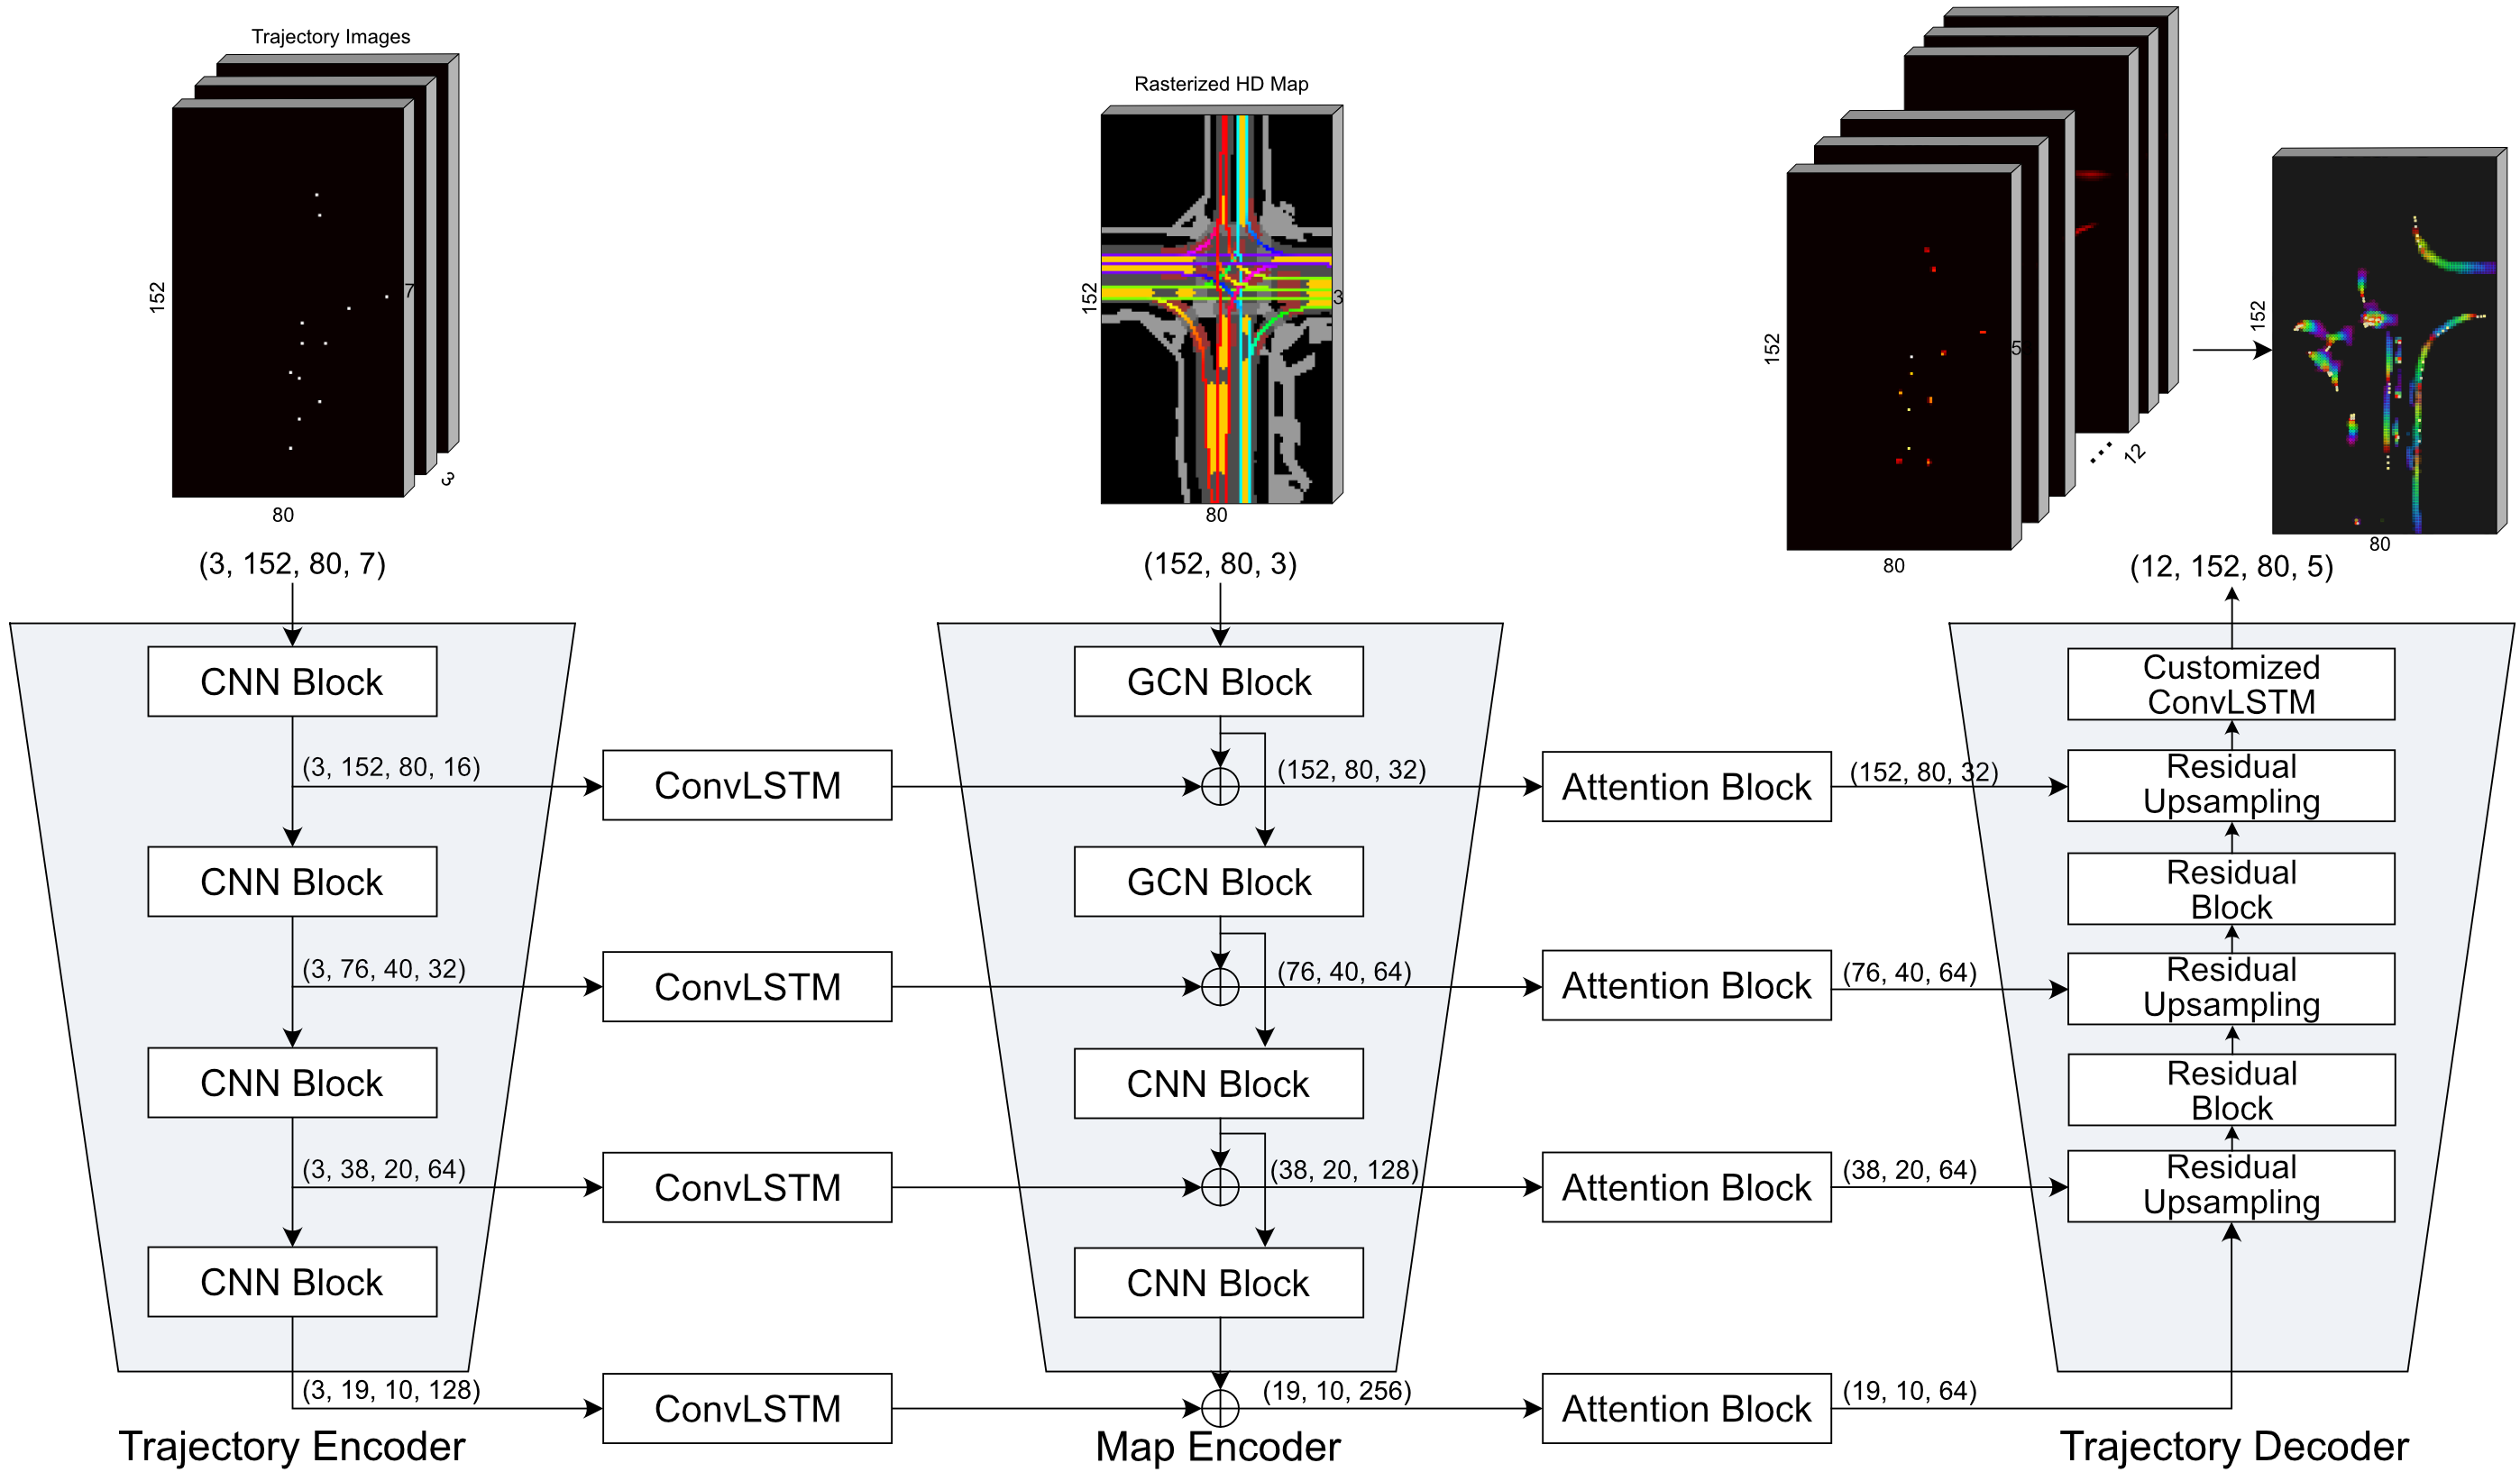
\includegraphics[width=\linewidth]{figures/caspnet_arch.png}
  \caption{CASPNet architecture overview: dual FPN encoders with Gabor filters, pixel-adaptive attention, and grid-based ConvLSTM decoder.}
  \label{fig:caspnet_overview}
\end{figure}

The CASPNet architecture is illustrated in~\autoref{fig:caspnet_overview} and consists of the following components:
\begin{description}[leftmargin=1em,itemsep=2pt]
\item[Dual FPN encoders.] Separate feature-pyramid networks process
\begin{enumerate}[label=\roman*)]
    \item a BEV stack of past agent trajectories \( \mathbf{I}_d\in\mathbb{R}^{T_p\times H\times W\times F_d} \)
    \item a static HD-map raster \( \mathbf{I}_s\in\mathbb{R}^{H\times W\times F_s} \)
\end{enumerate}

The map branch employs \emph{steerable Gabor filters}%
\footnote{See~\autoref{ssec:gabor_filters} for further details.}
in the first two convolutional blocks. These filters are particularly well-suited for processing structured environments like road networks, where lane markings, boundaries, and curbs exhibit strong orientation and scale-specific patterns. A Gabor filter combines a Gaussian envelope with a sinusoidal carrier wave, allowing it to simultaneously localize features in space and frequency. This makes it highly effective for detecting elongated and parallel structures across varying scales and rotations~\cite{steerableGaborFilters}.

At each level \( \ell \), the trajectory branch produces:
\begin{equation}
\label{eq:fpn_traj}
F^{\mathrm{traj}}_{\ell}(t) = \mathrm{CNN}_\ell\bigl(\mathbf{I}_{d}(t)\bigr)
\end{equation}
where all \( T_p \) BEV frames representing the agent trajectories are encoded independently by the same CNN, yielding a \emph{time-dependent} \emph{multi-scale feature map} \( F^{\mathrm{traj}}_{\ell}(t) \in \mathbb{R}^{C_\ell \times H_\ell \times W_\ell} \) at each pyramid level \(\ell\) and timestep \( t \in \{1,\dots,T_p\} \).\\
The static map branch uses so-called \emph{Gabor CNN blocks}~\cite{Luan2018GCNN} in the first two convolutional blocks to extract orientation-sensitive features, yielding a static feature map \( F_{\ell}^{\mathrm{map}} \in \mathbb{R}^{C_\ell \times H_\ell \times W_\ell} \) at each pyramid level.\\
The map features are computed as follows:
\begin{equation}
\label{eq:fpn_map}
\mathbf{F}_{\ell}^{\mathrm{map}}
= \mathrm{CNN}_\ell^{\circ}(\mathbf{I}_s) \quad \text{where } \circ = \begin{cases}
\mathrm{Gabor} & \text{if } \ell < 2, \\
\mathrm{Normal} & \text{otherwise }.
\end{cases}
\end{equation}

\item[Temporal fusion.] ConvLSTM cells at every pyramid level aggregate the temporal context across all \(T_p\) timesteps yielding a single feature map per level:
\begin{equation}
\label{eq:fpn_fusion_traj}
\mathbf{F}_{\ell}^{\mathrm{traj}}
= \mathrm{ConvLSTM}_\ell\Bigl\{\mathbf{F}^{\ell}_{d}(t)\Bigr\}_{t=1}^{T_p},
\end{equation}
which are then concatenated with the static map features at each level:
\begin{equation}
\label{eq:fpn_fusion}
\boldsymbol{\mathcal{F}}=\{\mathbf{F}_\ell^{\mathrm{traj}}\oplus \mathbf{F}_\ell^{\mathrm{map}}\}_{\ell=0}^{L-1}.
\end{equation}
\( \boldsymbol{\mathcal{F}} \) is the resulting latent feature pyramid.

\item[Pixel-adaptive attention.] The \emph{Attention Block} in the lateral skip connections in \autoref{fig:caspnet_overview} blends multiple \emph{dilated convolutions}\cite{dilatedConv21} per pixel, capturing short- and long-range interactions through learned per-pixel attention weights over different dilation rates. For each spatial location \((i,j) \in \{1,\dots,H^{\ell}\} \times \{1,\dots,W^{\ell}\}\), attention weights \(\alpha^{(i,j)}_{r}\) are computed over different dilation rates \( r \):
\begin{equation}
\label{eq:pixel_attention}
\mathbf{F}_{\ell, att}^{(i,j)} = \sum_{r} \alpha^{(i,j)}_{r} \cdot \text{DilatedConv}_r(\mathbf{F}^{(i,j)}_{\ell}),
\end{equation}
where \(\alpha^{(i,j)}_{r} = \text{softmax}(\text{Conv}(\mathbf{F}^{(i,j)}_{\ell})))\) are learned attention weights that allow the network to dynamically select appropriate receptive field sizes for each spatial location.

\item[Grid-based decoder.] The decoder employs a series of \emph{residual upsampling blocks} to progressively upsample the feature maps from the FPN to the original raster resolution. Each residual block consists of a parallel \emph{transposed convolution} and a \emph{linear interpolation} layer. The resulting feature maps of each upsampling block are concatenated with the corresponding feature maps the next level of the FPN.\\
Finally, the decoder uses a \emph{ConvLSTM} layer to autoregressively generate future predictions. For each future timestep \(t \in \{T_p, \ldots, T_p + T_f - 1\}\), the decoder outputs occupancy probabilities and motion offsets.

\paragraph{Pros.} Inference time independent of agent count; inherent multi-modality via heat-map superposition.\\
\paragraph{Cons.} Metric accuracy capped by raster resolution; inference cost scales with grid size; vectorized outputs require post-processing; No multi-modal prediction; limited temporal modeling; No explicit relationship modeling between agents or between agents and map; No symmetries in the agent-centric coordinate system for all but the ego agent.

%--------------------------------------------------------------------
%% Above is done %%
\subsubsection*{CASPFormer: Trajectory Prediction with Deformable Attention}
\label{ssec:caspformer}

retains CASPNet's multi-scale CNN backbone to encode rasterized BEV inputs into hierarchical feature maps. These are flattened into tokens at each scale and enriched with 2D sinusoidal position encodings before being passed into a \textbf{Deformable Self-Attention} layer that fuses multi-scale context at $\mathcal{O}(N)$ complexity~\cite{zhu2021deformabledetr}. The resulting fused tokens serve as the keys and values in the decoder, which autoregressively emits vectorized \((x,y)\) trajectories by employing a \textbf{Deformable Cross-Attention} module.

\begin{figure}[ht]
  \centering
  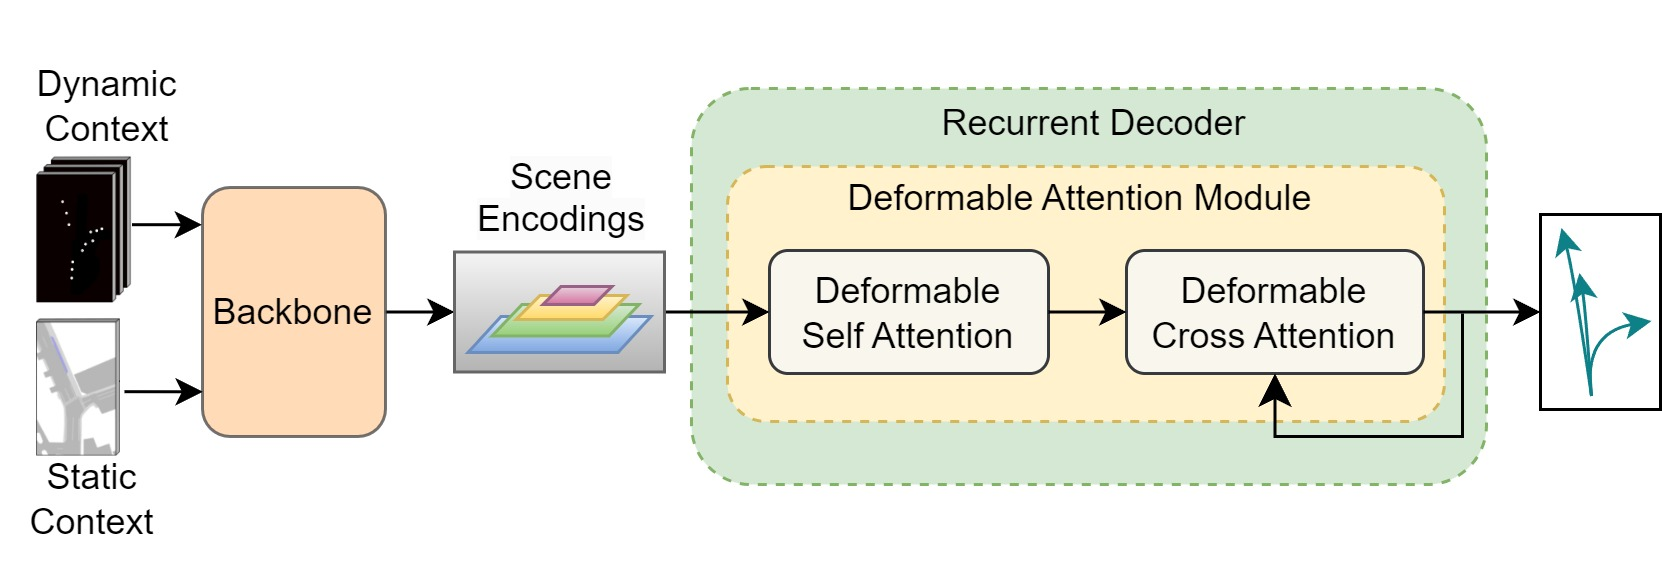
\includegraphics[width=\linewidth]{figures/caspformer-overall-arch.jpg}
  \caption{CASPFormer architecture: retains CASPNet's CNN backbone but replaces grid decoder with deformable attention transformer for vectorized trajectory output.}
  \label{fig:caspformer_overall}
\end{figure}


\begin{description}[leftmargin=1em,itemsep=2pt]
\item[Deformable Self-Attention (DSA).] The FPN feature maps \(\boldsymbol{\mathcal{F}} = \{\mathbf{F}_\ell\}_{\ell=0}^{L-1}\) are flattened and concatenated into a unified feature sequence as well as enriched with non-learnable 2D sinusoidal encodings to retain spatial relationships. DSA then performs feature fusion across multiple scales with \(\mathcal{O}(N)\) complexity.
\begin{equation}
\label{eq:msda_fusion}
\mathbf{Z} = \text{MSDA}(\text{Flatten}(\boldsymbol{\boldsymbol{\mathcal{F}} + \text{PE}})),
\end{equation}
where learned sampling offsets \(\boldsymbol{\Delta p}_{lkm}\) focus attention on the most informative spatial locations across pyramid levels. Each attention head \(m\) at level \(\ell\) samples \(K\) points around reference positions.

\item[Recurrent deformable cross-attention.] The core innovation lies in the autoregressive decoding scheme. For each future timestep \(t \in \{T_p + 1, \ldots, T_p + T_f\}\), dual queries attend to the fused features \(\mathbf{Z}\):
\begin{equation}
\label{eq:dual_query_update}
\begin{aligned}
\mathbf{Q}_t^{temp} &= \mathbf{Q}_{t-1}^{temp} + \text{PE}(\hat{\mathbf{p}}_{t-1}) \\
\mathbf{Q}_t^{mode} &= \text{Learnable}(\mathbb{R}^{M \times d}) \\
\mathbf{Q}_t &= \mathbf{Q}_t^{temp} \oplus \mathbf{Q}_t^{mode}
\end{aligned}
\end{equation}
where \(\mathbf{Q}_t^{temp}\) are temporal queries updated with positional encodings of previous predictions \(\hat{\mathbf{p}}_{t-1}\), and \(\mathbf{Q}_t^{mode} \in \mathbb{R}^{M \times d}\) are \(M\) learnable mode queries for multi-modal prediction.

The deformable cross-attention computes:
\begin{equation}
\label{eq:deformable_cross_attention}
\text{DeformAttn}(\mathbf{Q}_t, \mathbf{Z}) = \sum_{m=1}^{M} \mathbf{W}_m \sum_{k=1}^{K} A_{mkq} \cdot \mathbf{Z}(\phi(\mathbf{p}_q + \boldsymbol{\Delta p}_{mkq}))
\end{equation}
where \(A_{mkq}\) are attention weights, \(\boldsymbol{\Delta p}_{mkq}\) are learnable offsets, and \(\phi\) denotes bilinear sampling.

\item[Mixture-density head.] The final MLP outputs per-mode trajectory distributions as mixtures of Laplacian components:
\begin{equation}
\label{eq:mixture_output}
\begin{aligned}
\hat{\boldsymbol{\mu}}_{t,m}, \hat{\boldsymbol{\sigma}}_{t,m} &= \text{MLP}(\mathbf{Q}_t^{mode}) \\
\hat{\pi}_m &= \text{softmax}(\text{MLP}(\text{mean}(\mathbf{Q}_t^{mode})))
\end{aligned}
\end{equation}
yielding position means \(\hat{\boldsymbol{\mu}}_{t,m} \in \mathbb{R}^2\), uncertainty scales \(\hat{\boldsymbol{\sigma}}_{t,m} \in \mathbb{R}^2\), and mode probabilities \(\hat{\pi}_m\) for each of \(M\) modes.
\end{description}

The key innovation lies in the dual-query architecture that addresses mode collapse while maintaining temporal consistency. Unlike single-query approaches that struggle with behavioral diversity, the separation of temporal and mode queries enables CASPFormer to generate distinct trajectory modes while preserving smooth temporal dynamics.

\textbf{Pros.} Continuous, map-aligned trajectories; 30-40\% lower minFDE than CASPNet on nuScenes while training three times faster; complexity scales with prediction length \(\mathcal{O}(T_f)\), not grid size \(\mathcal{O}(HW)\); direct vectorized output without post-processing.
\textbf{Cons.} Still inherits quantization artifacts from the rasterized backbone; deformable attention adds modest per-step latency versus pure CNNs; requires careful hyperparameter tuning for attention sampling.

%--------------------------------------------------------------------
\subsection{Architectural Analysis and Comparison}
\label{ssec:comparison}

The evolution from CASPNet to CASPFormer illustrates key trade-offs in trajectory prediction architectures. We analyze these trade-offs across four critical dimensions:

\textbf{Representation paradigms.} CASPNet's fully rasterized approach treats trajectory prediction as a dense spatial problem, analogous to semantic segmentation. Every pixel potentially contains trajectory information, enabling inherent multi-agent modeling but limiting precision to grid resolution. CASPFormer's hybrid design preserves spatial reasoning in the encoder while switching to sparse, continuous decoding—combining the best of both paradigms.

\textbf{Computational complexity.} CASPNet's grid-based decoder scales as \(\mathcal{O}(HW \cdot T_f)\), making it suitable for edge deployment but memory-intensive for high-resolution scenes. CASPFormer's deformable attention achieves \(\mathcal{O}(N \cdot K \cdot T_f)\) complexity, where \(N\) is the number of query tokens and \(K\) is the sampling points per query (\(K \ll HW\)). This linear scaling with prediction horizon rather than spatial resolution makes CASPFormer more suitable for long-term prediction.

\textbf{Multi-modality mechanisms.} CASPNet achieves multi-modality through \emph{implicit} spatial distributions—multiple peaks in the occupancy heat-maps naturally represent different trajectory modes. However, this approach can suffer from mode blending and requires careful post-processing to extract clean trajectories. CASPFormer's \emph{explicit} mode queries provide cleaner mode separation and eliminate the need for trajectory extraction algorithms.

\textbf{Attention mechanisms.} Both architectures employ attention, but with different philosophies. CASPNet's pixel-adaptive attention operates densely across the entire spatial grid, learning local interaction patterns through dilated convolutions. CASPFormer's deformable attention is sparse and adaptive, focusing computational resources on relevant spatial locations through learned sampling offsets. This selective attention proves more efficient for capturing long-range dependencies while maintaining spatial precision.

\textbf{Future directions.} The progression from CASPNet to CASPFormer suggests several promising research directions: (1) \emph{End-to-end learning} that jointly optimizes perception and prediction modules, eliminating the rasterization bottleneck entirely; (2) \emph{Adaptive resolution} schemes that dynamically adjust spatial granularity based on scene complexity; (3) \emph{Temporal attention} mechanisms that model long-term dependencies more effectively than recurrent approaches; and (4) \emph{Multi-scale deformable attention} that operates directly on vectorized scene representations.

Both architectures demonstrate the evolution from grid-based to hybrid approaches in trajectory prediction, with CASPFormer representing a crucial stepping stone toward fully vectorized methods while maintaining the computational advantages of CNN backbones. The success of this hybrid approach validates the principle that combining proven architectural components (CNNs for spatial reasoning, transformers for sequential modeling) often outperforms end-to-end novel designs.

%--------------------------------------------------------------------
\subsection*{Summary}
This section provided a comprehensive overview of two seminal works in rasterized trajectory prediction: CASPNet's grid-based joint prediction and CASPFormer's hybrid CNN-transformer architecture. While both methods process BEV inputs, their architectural choices reflect different trade-offs between computational efficiency, prediction accuracy, and deployment constraints. CASPNet prioritizes constant-time inference and edge compatibility, while CASPFormer emphasizes prediction quality and continuous output representation. These design principles continue to influence modern trajectory prediction systems, including the query-centric approaches discussed in subsequent sections.

%--------------------------------------------------------------------
\newpage